\chapter{Teil von Jörg Hoffstetter}

\section{Anforderungen}

\subsection{Begriffe}
\begin{description}
	\item[Anforderungen:] Wünsche, Ziele und Vorgaben von Benutzer an ein System. Bedingungen und Eigenschaften des zu entwickelnden Systems.
	\item[Stakeholder:] Person oder Organisation die Einfluss auf die Anforderungen hat. (Bspw: Kunde, Vorschriften, Gesetze)
\end{description}

\subsection{Einführung}

Anforderungen können auf verschiedenen Abstraktionslevels beschrieben werden. Am ungenausten sind die \emph{Needs} (Was braucht der Kunde?).

Aus den \emph{Needs} können die Kundenanforderungen abgeleitet werden. Es sind problemorientierte Anforderungen (Was will der Kunde?), welche auch vom Kunden verstanden werden. Ein \emph{Feature} ist ein Merkmal eines Systems, welches ein oder mehrere Anforderungselemente betrifft.

Von den Kundenanforderungen (fachlich) werden die präzisen und widerspruchsfreien Softwareanforderungen (technisch) abgeleitet. Es sind lösungsorientierte Anforderungen für die Entwickler. Sie dienen als Grundlage für das spätere Design.

Zusätzlich zu den funktionalen Anforderungen (Was soll ein Produkt tun?) existieren die nichtfunktionalen Anforderungen. Beispiele für nichtfunktionale Anforderungen sind:
\begin{itemize}
	\item Performanz und Effizienz
	\item Zuverlässigkeit (Reliability) und Verfügbarkeit (Availability)
	\item Sicherheit (Security)
	\item Wartbarkeit (Maintainability)
\end{itemize}
Anforderungen sollten folgende Eigenschaften erfüllen:
\begin{itemize}
	\item Verständlichkeit, Klarheit
	\item Eindeutigkeit (keine Missverständnisse)
	\item Vollständigkeit
	\item Konsistenz
	\item Korrektheit
	\item Gültigkeit (Ist Anforderung aktuell?)
	\item Verfolgbarkeit / Traceability
	\item Testbarkeit / Prüfbarkeit
	\item Machbarkeit / Umsetzbarkeit
	\item Bewertet (Prio, Aufwand, Risiko, …)
\end{itemize}

\subsection{Anforderungsengineering}

Anforderungen dienen als Grundlage für den Architekturentwurf. Umgekehrt werden im Architekturentwurf auch
Erkenntnisse gewonnen, die Auswirkungen auf die Anforderungen haben (Machbarkeit, Kosten) können. In der Praxis stellen wir daher
eine starke Wechselwirkung zwischen der Anforderungsdefinition und dem Architekturentwurf fest, wie die Abbildung \ref{fig:anforderungsengineering} darstellt.
\begin{figure}[h!]
	\centering
	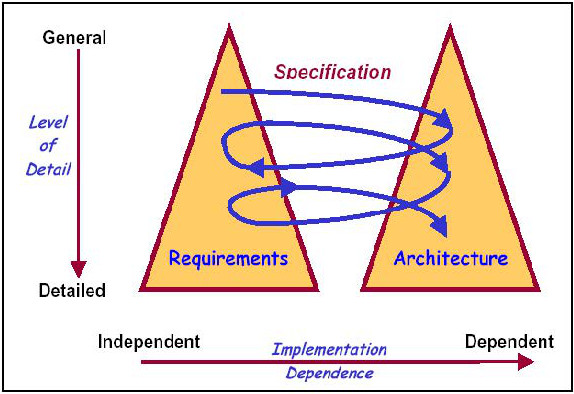
\includegraphics[width=0.7\linewidth]{fig/anforderungsengineering}
	\caption{Zusammenhang Anforderungen und Architektur}
	\label{fig:anforderungsengineering}
\end{figure}
Das Anforderungsengineering kann mit zwei Vorgehens-Modellen durchgeführt werden. Beim ersten Modell wird das Anforderungsengineering als Projektphase durchgeführt. Dabei kann jedoch auf Anforderungs-Änderung erst spät reagiert werden und der Kunde ist nicht zufrieden. Bei Modellen wie SoDa oder Scrum werden die Anforderungen kontinuierlich (just in time) erhoben. Am Anfang eines Projektes definiert man die Anforderungen nur grob und geht zusammen mit dem Kunden immer mehr ins Detail.

\begin{figure}[h!]
	\centering
	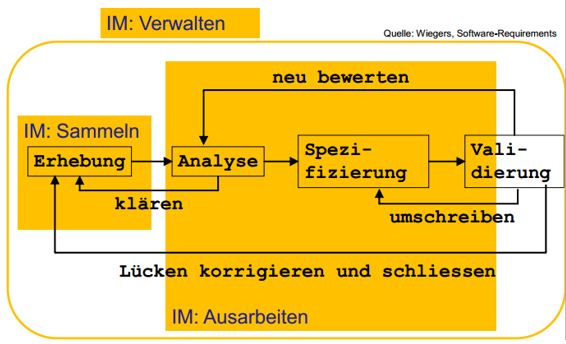
\includegraphics[width=0.7\linewidth]{fig/anforderungsengineering-prozess}
	\caption{Anforderungsengineering Prozess}
	\label{fig:anforderungsengineering-prozess}
\end{figure}

\subsection{Anforderungs-Techniken}

Anforderungen könne aus verschiedenen Quellen (Stakeholder, Dokumente usw.) und mit verschiedenen Ermittlungstechniken erhoben werden. Um diese Anforderungen festzuhalten werden folgende Techniken eingesetzt:
\begin{description}
	\item[Systemkontext:] Abgrenzung des Produktumfanges (Kontextdiagramm)
	\item[Ziele:] Es werden die Intentionen der Kunden festgehalten (keine Lösungsansätze dokumentieren)
	\item[Szenarien:] exemplarische, konkrete Abläufe festhalten (z.B. in Form von Use Cases, Szenario-Beschreibungen, User-Story)
	\item[Geschäftsregeln:] Regeln für unternehmerische Entscheidungen z.B. in Form von Entscheidungstabellen
	\item[Lösungsorientierte Anforderungen:] Datenstrukturen, Verhalten, Funktionssicht eines Systems, Schnittstellenbeschreibungen usw.
\end{description}
Mit einem Kontextdiagramm wird das System und dessen Kontext klar abgegrenzt. Typische Inhalte eines Kontextes sind Personen, technische Systeme oder Prozesse. Die Systemgrenze separiert das geplante System von seiner Umgebung (Lieferumfang). Möchte man ein Kontextdiagramm erstellen muss zuerst die Systemgrenze festgelegt werden. Danach sollte überlegt werden was alles zum Kontext gehört um anschliessend die Kontextgrenze festlegen zu können. Am Schluss wird noch der Nachrichtenfluss zwischen dem System und dem Kontext über Schnittstellen festgelegt. Es geht darum auch aufzuzeigen was nicht Teil des zu entwickelnden Systems ist (Definition des Lieferumfangs)!

\subsection{Anforderungen mit Use Cases festhalten}

Use Cases sind eine Technik um Anforderungen festzuhalten. In einem Use Case wird textuell eine Sequenz von Interaktion zwischen dem Benutzer und dem System beschrieben (als Text oder als Flussdiagramm). Dieser Ablauf sollte dem Benutzer einen Nutzen bringen. Auch allfällige Sonderfälle werden beschrieben. Use Cases können überarbeitet und verfeinert werden z.B. durch Pre-/Post-Condition, alternative flows oder nichtfunktionale Anforderungen. Use Cases eignen sich gut um mit dem Kunden wichtige Abläufe durchzugehen.

Sämtliche Use Cases und Benutzer eines Systems werden in einem Use Case Diagramm zusammengefasst. Mit Pfeilen kann festgelegt werden ob ein Benutzer einen Use Case auslöst oder von einem Use Case benötigt wird. Abbildung \ref{fig:use-case-diagramm} zeigt ein Use Case Diagramm.
\begin{figure}
\centering
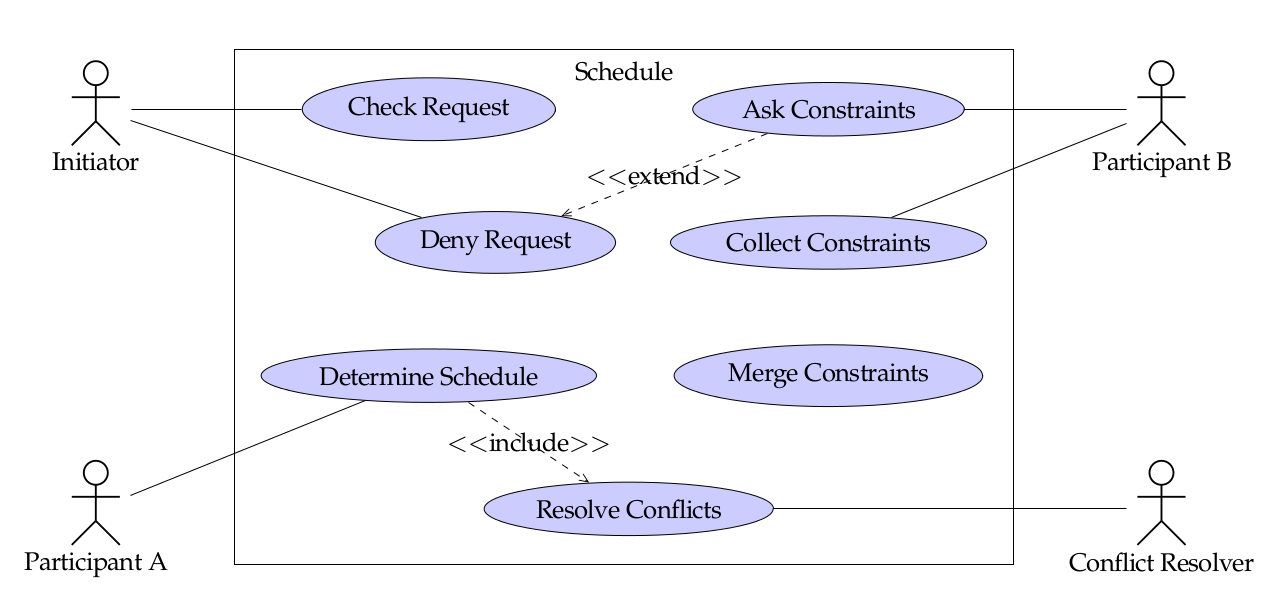
\includegraphics[width=\linewidth]{fig/use-case-diagramm}
\caption{Use Case Diagramm}
\label{fig:use-case-diagramm}
\end{figure}

\paragraph{Best Practices} Verwende keine includes oder excludes. Uses Cases werden unnötige kompliziert. Use Cases können schlussendlich auch mit BPM, EPK oder Aktivitätsdiagramme modelliert werden, denn es sind Abläufe.

\subsection{Anforderungen textuell festhalten}

Alternativ zu den Use Cases können Anforderungen auch rein textuell festgehalten werden. Eine Möglichkeit wäre die Feature-Liste. Dabei werden alle Anforderungen in einer Tabelle festgehalten und evtl. mit Priorität, Aufwand oder Risiko ergänzt. Die Features können auch detailliert werden und in Unter-Feature zerlegt werden. Eine weitere Möglichkeit Anforderungen textuell festzuhalten sind User Stories wie sie in Scrum verwendet werden. User Stories werden aus Benutzersicht geschrieben und haben immer folgendes Format:
\begin{quote}
	As a \emph{user role}, I need a \emph{functionality}, so that I get \emph{business value}
\end{quote}
Zu jeder User Story gehören Akzeptanzkriterien um die Vollständigkeit zu garantieren. Gute User Stories sind INVEST:
\begin{tabbing}
	\hspace{3cm}\=\kill
	\textbf{I}ndependent: \> möglichst unabhängig voneinander \\
	\textbf{N}egotiable: \> zerlegbar, komponierbar, änderbar, verhandelbar \\
	\textbf{V}aluable: \> hat wirtschaftlichen Wert \\
	\textbf{E}stimatable: \> so klar, dass es vom Team geschätzt werden kann \\
	\textbf{S}mall: \> klein genug, um in einem Sprint entwickelt werden zu können \\
	\textbf{T}estable: \> klare Akzeptanzkriterien 
\end{tabbing}
User Stories lassen sich auf drei Arten zerlegen (detaillieren):
\begin{enumerate}
	\item Nach Daten
	\item Nach Benutzer/Rollen
	\item Nach Prozessschritten
\end{enumerate}

\subsection{Anforderungen mit Modellen festhalten}

Anforderungen lassen sich auch mit Modellen darstellen. Durch eine objektorientierte Analyse (OOA) lässt sich ein Fach- oder Domänenmodell erstellen. Dieses Modell beschreibt das Anwendungsgebiet (Domäne) der Software in der Sprache des Benutzers und fokusiert sich dabei auf die Fachobjekte (Entitäten). Dargestellt wird es beispielsweise in UML oder wie in Abbildung \ref{fig:komisches-modell-ohne-namen}.
\begin{figure}
	\centering
	\begin{subfigure}[b]{0.4\textwidth}
		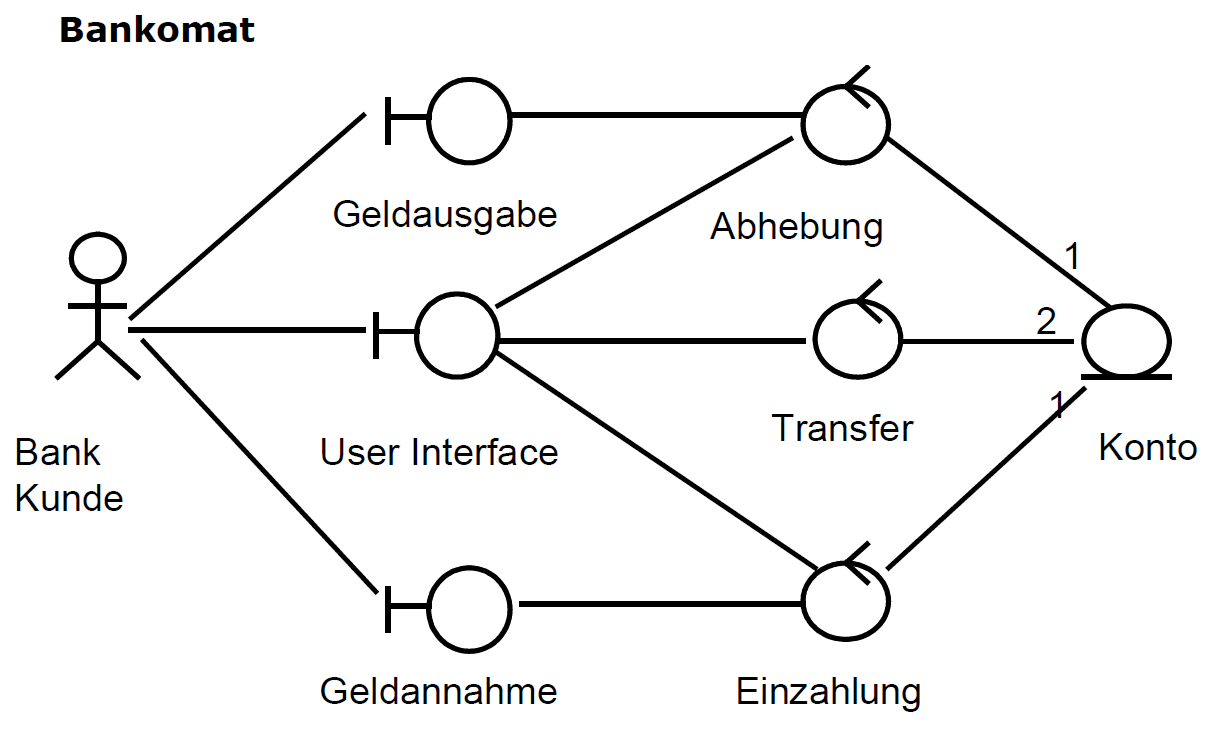
\includegraphics[width=\linewidth]{fig/komisches-modell-ohne-namen-1}
	\end{subfigure}
	\begin{subfigure}[b]{0.5\textwidth}
		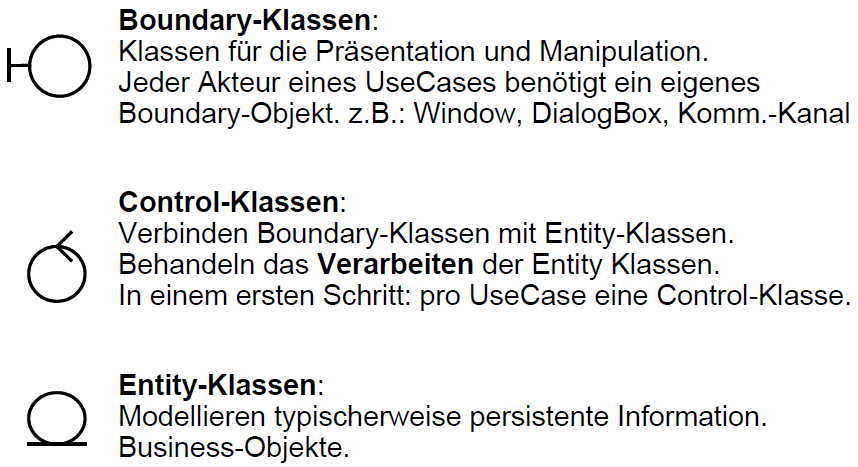
\includegraphics[width=\linewidth]{fig/komisches-modell-ohne-namen-2}
	\end{subfigure}
	\caption{Komisches Modell ohne Namen}
	\label{fig:komisches-modell-ohne-namen}
\end{figure}
Für dynamische Anforderungen können Sequenzdiagramme verwendet werden. Diese Modelle beschreiben Anforderungen und keine Lösungen.

\subsection{Prototypen}

Prototypen werden zu verschiedenen Zwecken erstellt:
\begin{itemize}
	\item Experimenteller Prototyp: zur Beurteilung bestimmter Problemlösungen. Ziel ist es nachzuweisen, dass Spezifikationen oder Ideen tauglich sind.
	\item Prototyp als Teil der Produkt-Definition (GUI-Protoyp).
	\item Evolutionäres Prototyping: Der Prototyp ist funktionsfähig und wird bis zur Produktreife weiterentwickelt (Scrum). 
\end{itemize}
Es gibt zwei Typen von Prototypen:
\begin{description}
	\item[Vertikale Prototypen:] Es werden nur bestimmte Funktionen über alle Layers getestet (Machbarkeit)
	\item[Horizontale Prototypen:] Es wird nur von einem Layer ein Prototyp erstellt (z.B. GUI)
\end{description}
Durch Prototypen ergeben sich folgende Vor-/Nachteile:
\begin{itemize}
	\item[+] Reduktion der Entwicklungsrisiken
	\item[+] Kreativität, neue Lösungsansätze
	\item[+] GUI-Prototyp: Ideal für die Diskussion mit Kunde
	\item[--] Kosten
	\item[--] Illusion nach Aussen: Projekt bereits fertig
\end{itemize}

\subsection{Dokumentation von Anforderungen}

Da Anforderungsdokumente als Grundlage für die Projektplanung, Kostenschätzung, Implementierung, Testen usw. dienen, müssen sie gewissen Qualitätskriterien erfüllen. Diese Kriterien sind nachfolgend aufgelistet:
\begin{itemize}
	\item Eindeutigkeit und Konsistenz
	\item Klare Struktur
	\item Erweiterbarkeit
	\item Vollständigkeit
	\item Verfolgbarkeit (Traceability) der Beziehungen unterschiedlicher Dokumente (inkl. Code)
\end{itemize}
Um diese Kriterien zu erfüllen wurden verschiedene Normen und Empfehlungen erstellt. Bei der DIN-Norm wird vom Kunden ein Lastenheft und vom Lieferant ein Pflichtenheft verlangt. Auch das IEEE stellt mit der SRS 830 eine Dokumentenvorlage für Anforderungen zur Verfügung.

\subsection{Anforderungen verwalten}

Um Anforderungen besser verwalten zu können sollten folgende Punkte beachtet werden:
\begin{itemize}
	\item Priorisierung
	\item Verfolgbarkeit (Traceability), die Fähigkeit eine Anforderung über den gesamten Lebenszyklus des Systems hinweg zu verfolgen (Dokumente und Code)
	\item Verwaltung von Anforderungsänderungen
	\item Anforderungen mit Attributen versehen (ID, Name, Beschreibung, Version, Autor, Quelle, Priorität, Kritikalität) 
\end{itemize}

\subsection{Use Case vs. User Story}
Ersetzt das eine das andere? Nein. Es sind zwei unterschiedliche Dinge. Use Cases werden detailliert beschrieben und sind eher schwergewichtige Dokumentationsinstrumente. User Stories dienen eher zur Besprechung und auch als leichtgewichtige Planungsinstrumente. Prominente Methodiker wie Martin Fowler gehen davon aus, dass es zwei verschiedene Instrumente sind, welche sich ergänzen können\footnote{\href{http://blog.hood-group.com/blog/2013/05/15/use-cases-und-user-stories-verbundete-oder-feinde/}{http://blog.hood-group.com/blog/2013/05/15/use-cases-und-user-stories-verbundete-oder-feinde/}}.

\subsection{Features vs. Use Cases}
Use Case ist eine Überlegung eines Ablaufs. Erst beim Ablauf kommt man auf die Features.

\subsection{RUP vs SODA}
RUP ist Use Case-orientiert wohingegen Soda Story-orientiert ist.

\section{Planung}

\subsection{Rahmenplan}

Der Rahmenplan wird in der Initialisierungsphase erstellt und die Meilensteine definiert. Ein grosses Risiko in einem Projekt stellen neue Technologien dar. Deshalb sollten diese möglichst früh mit einem Prototypen überprüft werden

\begin{figure}[h!]
\centering
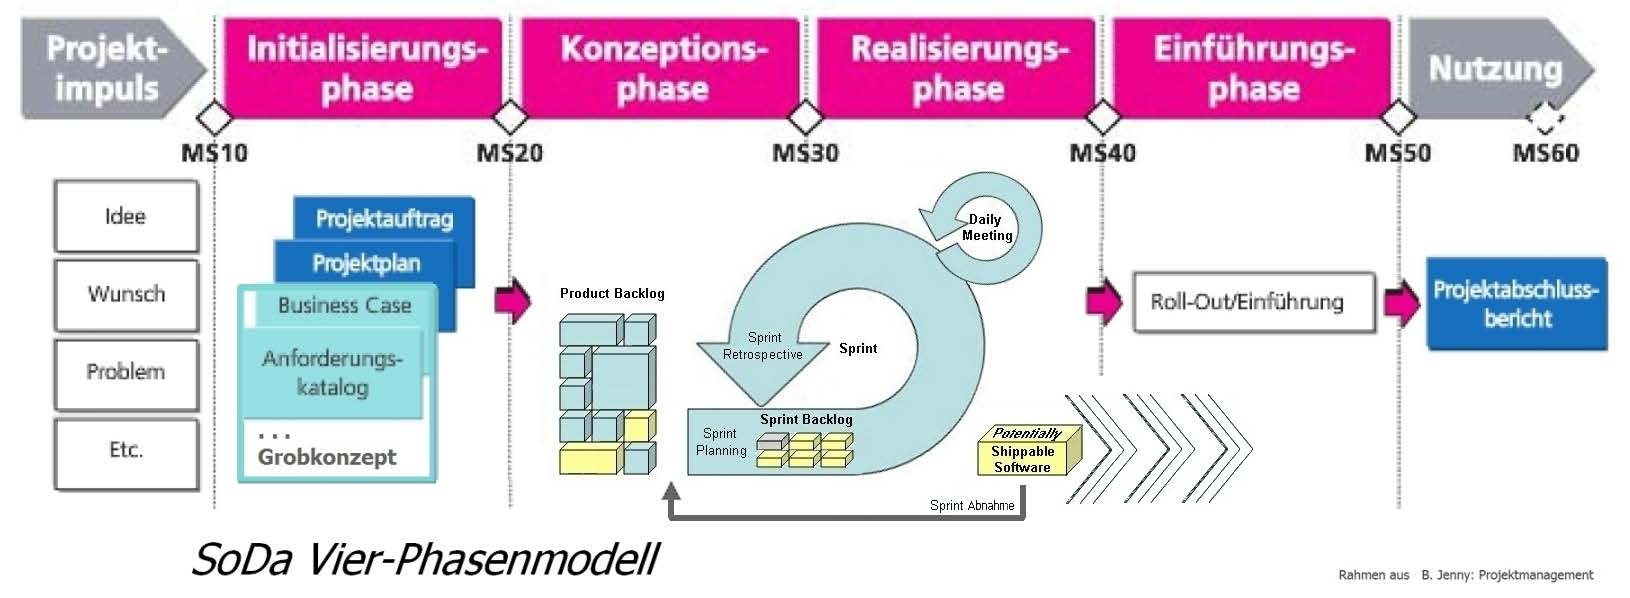
\includegraphics[width=0.8\linewidth]{fig/rahmenplan}
\caption{Rahmenplan SODA}
\label{fig:rahmenplan}
\end{figure}

Ein Meilenstein ist eine Verknüpfung von messbaren Ergebnissen zu einem definierten Zeitpunkt. Meilensteine dienen der Überwachung des Projektes und dem Einleiten von notwendigen Massnahmen. Wird folglich ein Meilenstein nicht erreicht, muss man sich über einen Projektabbruch Gedanken machen.

\subsection{Scrum}

Der Inhalt eines Sprints plant man definitiv bevor man den Sprint beginnt. Der übernächste Sprint wird grob geplant. Ein Sprint enthält typischerweise drei bis sechs Userstories. Das Resultat eine Sprints muss ein \emph{potentially shippable product} sein. Das heisst die Software entspricht den Anforderungen und ist getestet. Zudem ist die Software integriert und funktioniert auf einer realitätsnahen Umgebung. Stories sollten primär neue Funktionen beschreiben. Unterstützungstätigkeiten (Konzepte, Tests, Dokumente usw.) sollten als Tasks innerhalb der Stories definiert werden.

Der Product Owner ist verantwortlich für das Produkt. Er ist die Schnittstelle zum Kunden und erstellt aufgrund dessen die Anforderungen. Da er auch für den wirtschaftlichen Erfolg des Produktes verantwortlich ist, misst er den Projektfortschritt und führt die Akzeptanztests durch. Zudem priorisiert er die Anforderungen aus dem Backlog und definiert mit dem Team die Sprintinhalte.

Der Product Backlog ist eine geordnete Liste mit allem, was in dem Produkt benötigt werden könnte. Er ist die einzige Quelle für Anforderungen. Er enthält zudem unkritische Bugs (kritische in Sprint Backlog) und Spikes (Forschungsaufträge). Ein guter Backlog ist \textbf{DEEP}:
\begin{itemize}
	\item \textbf{D}etailed Apropriately (angemessen Detailliert)
	\item \textbf{E}stimated (Geschätzt)
	\item \textbf{E}mergent (Entwickelt sich, wird gepflegt)
	\item \textbf{P}rioritized (Priorisiert)
\end{itemize}
Der Product Backlog besteht aus Backlog-Items. Zu jedem Backlog-Item gehören Akzeptanzkriterien. Ein Backlog-Item kann ein Epic, eine User Story oder ein sonstiges Work Item sein (Bugs, Spikes, Doku oder Infrastruktur). Der Sprint Backlog enthält für jeden öffentlich alle Anforderungen, Tasks und kritische Fehler für den Sprint.

Ein Sprint gliedert sich in eine Sprint Planung, der Sprint Durchführung und dem Sprint Abschluss. 
Bei der Sprint Planung stellt der Product Owner das Sprint-Ziel und wichtige Anforderungen vor. Das Team wählt und schätzt die Anforderungen zusammen mit dem Product Owner. Danach plant das Team die einzelnen Task der Anforderungen. Die Planung darf jedoch nicht überhand nehmen.
Bei der Sprint Durchführung arbeitet das Team Tasks aus dem Sprint Backlog ab. Fertige Anforderungen werden zur Kontrolle auf dem Burn-Down Chart vermerkt. Der Produkt Qwner nimmt die fertigen Anforderungen ab. 
Der Sprint Abschluss wird zusätzlich noch in einen Sprint Review und einer Retrospektive unterteilt. Der Sprint Review ist eine öffentliche Veranstaltung auch für den Kunden. Am besten lädt man den Kunden direkt ein zum Sprint Review. Die fertige Anforderungen werden vorgeführt. Bei der Retrospektive reflektiert das Team den letzten Sprint. Gutes wird beibehalten und Probleme werden behoben.

\begin{figure}
\centering
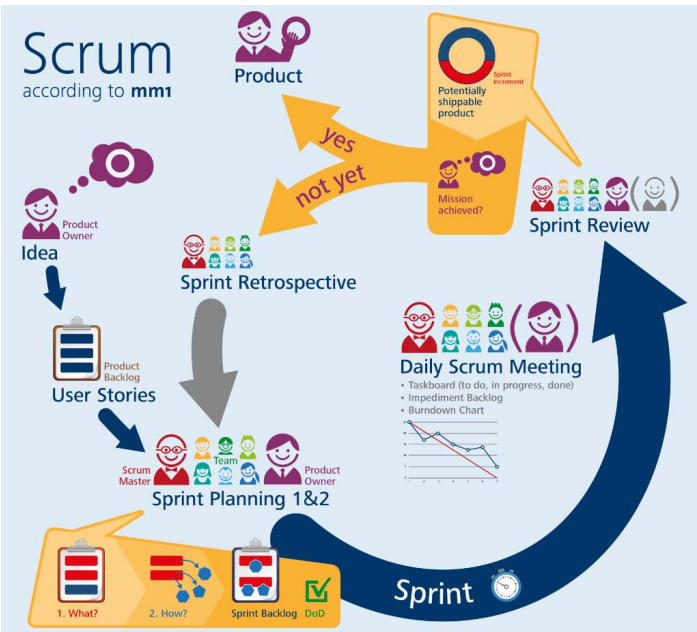
\includegraphics[width=0.7\linewidth]{fig/scrum-lifecycle}
\caption{Scrum Lifecycle}
\label{fig:scrum-lifecycle}
\end{figure}

\textbf{Scrum Master:} Ist einer der drei Kernrollen in Scrum. Er wacht darüber, dass die Scrum Regeln eingehalten werden. Ausserdem schaut ein guter Scrum Master zu seinem Team - er motiviert es, erwägt Alternativen oder überdenkt Prioritäten. Aber am wichtigsten ist, dass er sich um die Dinge kümmert, welche das Team davon abhalten optimal zu arbeiten.

\textbf{Definition of Done (DoD):} Ist ein Scrum-Artefakt, welches beschreibt, wann eine Arbeit erledigt ist. Diese DoD lebt und wird sich im Verlauf des Projektes erweitern und dies in der Regel in der Sprint Retro. Die DoD kann sich auf unterschiedliche Dinge beziehen. Auf Backlog-Items, auf gewisse Tasks usw. Beispiel einer DoD:

\begin{itemize}
	\item Dokumentation aktualisiert (SysSpec).
	\item Code ist implementiert und auf der DEV Umgebung integriert.
	\item Code wurde durch einen zweiten Entwicklicker reviewed.
\end{itemize}

\begin{figure}
\centering
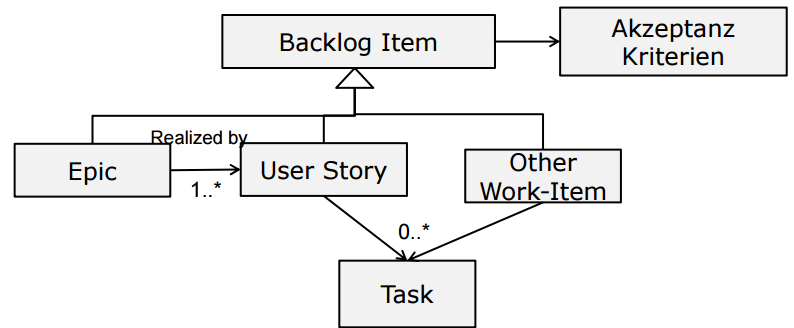
\includegraphics[width=0.7\linewidth]{fig/backlogitems}
\caption{Backlogitems}
\label{fig:backlogitems}
\end{figure}

\section{Modellieren}
Modellieren ist eine wichtige Tätigkeit. Man modelliert aus mehreren Gründen: Dokumentation, Verständnis- und Konsensbildung oder gesetzliche Vorgaben.

Es ist stets darauf zu Achten, dass man die richtige Flughöhe besitzt. Man spricht von \emph{Level of abstraction}. Zu Projektbeginn interessiert es niemanden, ob die Toilette im WC gelb oder grün wird. 

Oft ist das Modelliert ungleich dem Implementierten. Darauf sollte man immer bedacht sein und vorab vielleicht mal zuerst die Implementierung anschauen. Und in einem Konsistenzcheck eine Soll und Ist Gegenüberstellung machen.

\subsection{Begriffe}
\begin{itemize}
	\item \textbf{Modell} Ein Modell ist eine Abstraktion (Vereinfachung).
	\item \textbf{Diagramm} Möglichkeit ein Modell aus unterschiedlichen Sichten grafisch darzustellen.
\end{itemize}

\subsection{Modell-Typen}
Grundsätzlich unterscheidet man zwischen statischen und dynamischen Modellen. Ein statisches Modell beschreibt die Struktur, den Aufbau eines Systems (Uses-Beziehungen, part-of Zerlegung, Layer und Schichten, Verteilung)). Ein dynamisches Modell beschreibt wie das System interagiert, wie es lebt  (Daten- und Kontroll-Fluss, ausführbare Einheiten, Parallelität).

Man modelliert auf unterschiedlichen Ebenen. Auf der Konzept-Ebene geht es dabei um Analyse und Anforderungen. Auf der Ebene der Architektur will man die Komponenten-Beziehungen und Layer aufzeigen. Und auf Implementations-Ebene modelliert man den Code. Siehe dazu Abbildung \ref{fig:modelltypen}.

\begin{figure}[h!]
\centering
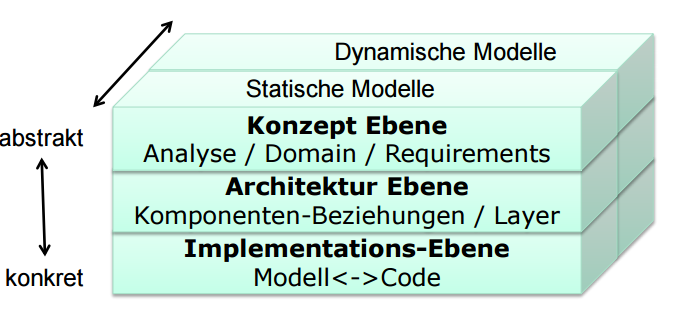
\includegraphics[width=0.7\linewidth]{fig/modelltypen}
\caption{Modell-Typen}
\label{fig:modelltypen}
\end{figure}

\subsection{Datenfluss vs. Kontrollfluss}
Der Kontrollfluss bezieht sich auf die zeitliche Abfolge der einzelnen Befehle. Der Datenfluss konzentriert sich auf die zeitliche Abfolge des Datenaustausches. Beide sind grundsätzlich gerichtet. Bsp: Datenfluss- und Kontrollfluss können in einer Aktion auch unterschiedliche Richtungen haben. Denke dabei an eine Getter-Methode wie int getZahl().

\begin{figure}[h!]
	\centering
	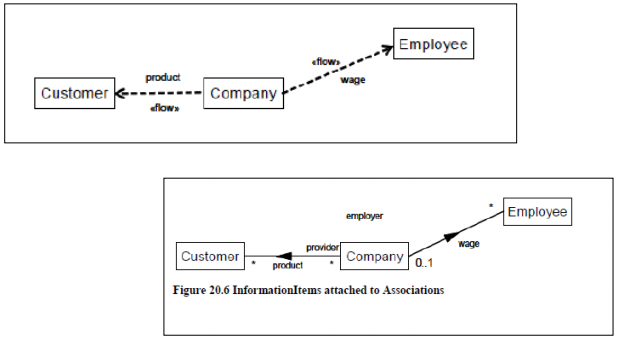
\includegraphics[width=0.7\linewidth]{fig/uml-datenfluss}
	\caption{UML Datenfluss}
	\label{fig:uml-datenfluss}
\end{figure}

\subsection{Architektursichten (Views)}
\begin{itemize}
	\item \textbf{Funktionale- / Konzeptionelle Sicht} Zerlegung in einzelne Komponente. Diagramme: Blockdiagramm, Komponentendiagramm 
	\item \textbf{Entwicklungs-Sicht} Statische Modul-Strukturen. Diagramme: Klassen- und Paketdiagramm. 
	\item \textbf{Verteilungs- / Betriebssicht} Zuordnung von Komponenten/Module zu physikalischen Ressourcen. Beschreibt wie das System administriert, betrieben und unterhalten wird. Diagramm: Verteilungsdiagramm
	\item \textbf{Datenstrukten} Konzeptionelle Datenstrukturen. Diagramme: Analyse-Modell, ERM. 
\end{itemize}

Beispiel eines funktionalen Blockdiagramm:
\begin{figure}[h!]
\centering
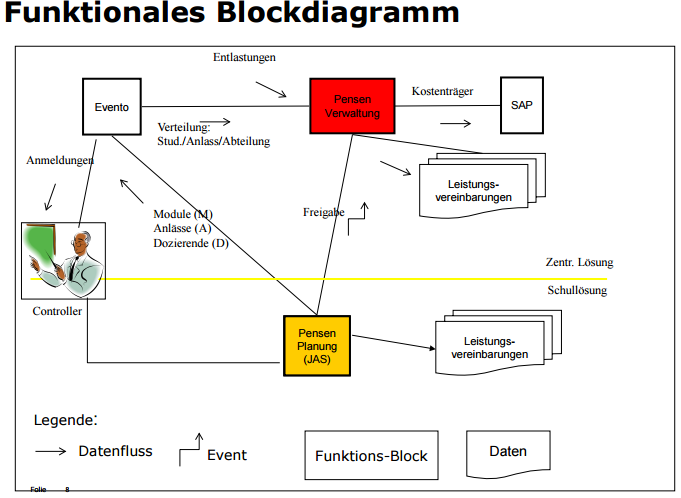
\includegraphics[width=0.8\linewidth]{fig/funktionales-blockdiagramm}
\caption{Funktionales Blockdiagramm}
\label{fig:funktionales-blockdiagramm}
\end{figure}

\subsection{Abhängigkeiten}
Eines der schwierigsten Themen der Informatik. Das Ziel ist immer eine möglichst lose Kopplung. Das erreicht man damit, dass man die Anzahl an Abhängigkeiten gering hält und allfällige Abhängigkeiten mit schwachen Formen umsetzt. Falls Klasse A von Klasse B abhängig ist, zeichnet man einen gestrichelten Pfeil von A nach B.

\begin{itemize}
	\item \textbf{Class Dependency} Klasse A nutzt Klasse B.
	\item \textbf{Interface Dependency} Klasse A nutzt keinen konkrete Klasse B sondern den Interface-Typ der Klasse B (schwächere Kopplung).
	\item \textbf{Compile-Time / Runtime-Depedency} Klasse A benötigt zur Kompliation ein Interface-Typ, die konkrete Implementierung wird erst zur Runtime relevant.
	\item \textbf{Indirect Dependency} Klasse A nutzt Klasse B. Klasse B nutzt Klasse C. Klasse A ist indirekt abhängig von Klasse C. (Auch bekannt als transitive Abhängigkeit).
\end{itemize}

\subsection{Assoziation}
Eine spezielle Form der Abhängigkeit. Klasse A hat eine Assoziation zur Klasse B, wenn A eine Membervariabel hält mit dem Typ von B. Man zeichnet von A nach B eine durchgezogene Linie.

\subsection{Paketdiagramme}
Pakete sind Ansammlungen von irgendwelchen Modellelementen. Mittels Paketen wird ein komplexes System in kleinere, überblickbare Einheiten gegliedert. Ein bestimmtes Modellelement gehört genau zu einem Paket.

\subsection{Zyklische Abhängigkeiten}
Wenn A von B abhängig ist und B von A. Oder wenn A von B und B von C und C wiederum von A. Dann haben wir Zyklen. Das erhöht die Kopplung des System und ist schlecht wartbar. Zyklen konnen oft mittels eines dritten vermieden werden. Der Dritte entkoppelt die beiden voneinander. In Java wird oft das Observer-Pattern eingesetzt.

\subsection{Weitere Modellierungen}

\begin{figure}[h!]
	\centering
	\begin{subfigure}[b]{0.4\textwidth}
		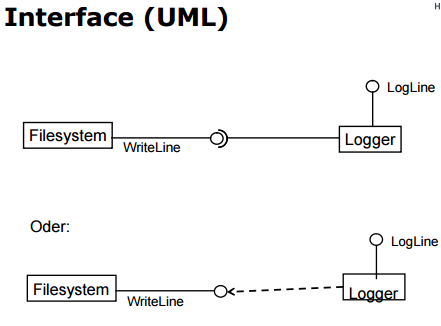
\includegraphics[width=\textwidth]{fig/interface-uml}
		\caption{Interface in UML}
		\label{fig:interface-uml}
	\end{subfigure}
	~
	\begin{subfigure}[b]{0.4\textwidth}
		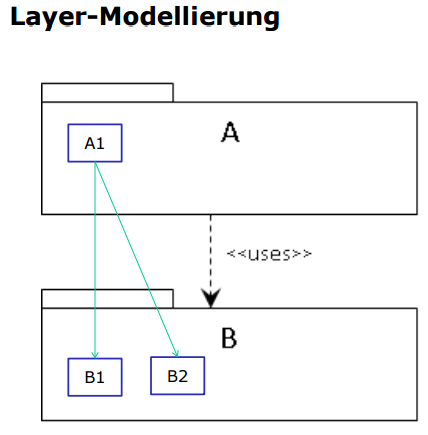
\includegraphics[width=\textwidth]{fig/layer-modellierung}
		\caption{Layer-Modellierung}
		\label{fig:layer-modellierung}
	\end{subfigure}
	\caption{Weitere Modellierungen}
	\label{fig:weitere-modellierungen}
\end{figure}

\subsection{Software Architektur Dokument}
SAD nach Pavlo Baron. In einem SAD werden Topics (protokollierte Architekturentscheide) und Sichten (unterschiedliche Brillen auf die Architektur) beschrieben. 
Ein Topic beinhaltet folgendes:

\begin{itemize}
	\item Zusammenfassung der Lösung
	\item Betroffene, relevante bzw. erfüllte Architekturfaktoren
	\item Lösung selbst, was wurde entschieden?
	\item Motivation: Warum wurde etwas entschieden?
	\item Ungelöste Punkte
	\item Betrachtete Alternativen, und warum diese verworfen wurden.
\end{itemize}
